\documentclass[acmtog]{acmart}
\usepackage{algorithm}  
\usepackage{algorithmicx}  
\usepackage{algpseudocode}
\usepackage{amsmath}
% Title portion
\title{Assignment 2 : Rigid body dynamics simulation} 
\author{Name:\quad Tianyuan Wu  \\ student number:\quad 63305667
	\\email:\quad wuty@shanghaitech.edu.cn}

% Document starts
\begin{document}
\maketitle

\vspace*{2 ex}


\section{Introduction}
	In this assignment, I implemented an simple engine for rigid body dynamics simulation.
	The implementation is in C++14 with OpenGL. It's worth mentioning that this engine is \textbf{all implemented 
	by me}, without any 3rd party libraries for calculation or rendering (except OpenGL). The workflow of this engine can 
	be described as:
	\begin{enumerate}
		\item Add objects (rigid bodies)
		\item Set initial configuration of rigid bodies
		\item Begin simulation (integration)
		\item Collision detection (using SAT Theorem)
		\item Collison handling 
		\item Simulation by integration...
	\end{enumerate}
	In my implementation, a general BasicShape class is provided, all shapes (Sphere, Cube, etc) 
	can derive from this class. Also, a general \texttt{RigidBody} class is provided for the simulation.
	For every \texttt{RigidBody}, we can add velocity ($v$), angular velocity ($\omega$), force($F$) and torque($\tau$) to it, 
	and the animation (result of simulation) can be automatically generated. What's fancy is, all implementation
	is done using templates, which means it's very easy to implement the simulation for other shapes once 
	related API is provided.\\
	For collision detection, I used a SAT Theorem based implementation, which can handle the collision
	between cubes well in practice.\\
	For collision contact handling, my implementation will first calculate the normal of the face where the collision
	occurred. Then, the impluse $J$ of this collision will be calculated. Finally, we will put apply this 
	impluse for both objects, and re-calculate the velocity and angular velocity.
	Here is a screenshot of the my implementation.\\
	All of these functions are tested under \texttt{macOS 10.15}, with \texttt{Apple clang 12.0.0}.
	\begin{figure}[H]
		\centering
		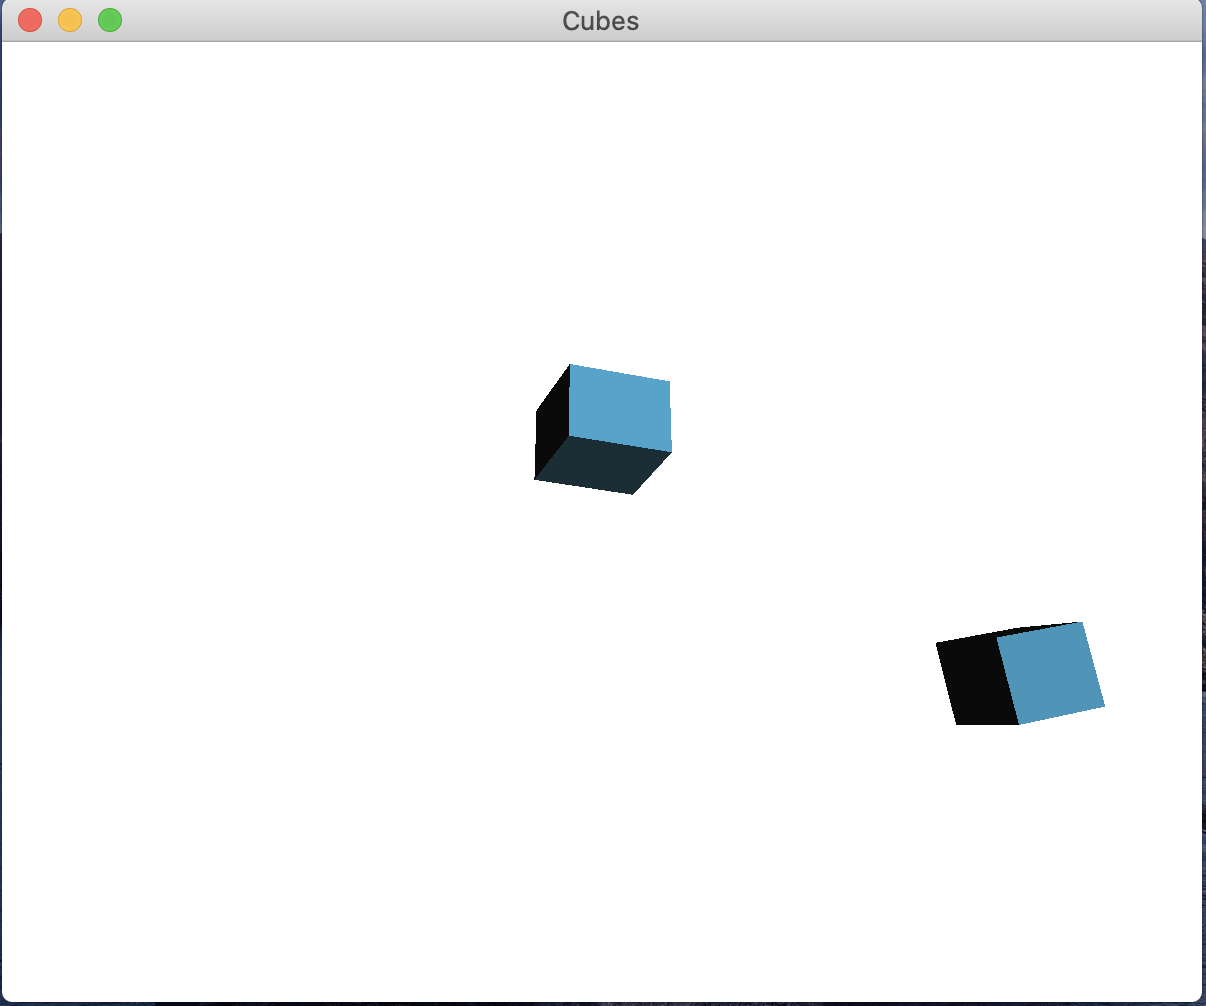
\includegraphics[scale=0.2]{sc1.png}
		\caption{Screenshot of my implementation}
	\end{figure}

\section{Implementation Details}
The implementation of this engine can be described in 3 parts: (1) Basic rigid body dynamics without 
collision handling; (2) Collision detection; (3) Collision contact handling.
\subsection{Basic rigid body dynamics}
In my implementation of rigid body dynamics, every rigid body hold its own velocity ($v$), angular velocity
 ($\omega$), force($F$) and torque($\tau$). Every rigid will update its position and orientation in \texttt{update()}
 funtion. The simulation process can be described by the following pseudo code:
\begin{algorithm}
	\caption {Simulation process}	
	\begin{algorithmic}[1]
		\While {true}
			\For{object : rigidBodies} 
				\State object.update();
				\State object.show();
			\EndFor
			ShowObjectsOnWindow();
		\EndWhile
	\end{algorithmic}
\end{algorithm}
In \texttt{update()} function, we need to re-calculate the velocity by given force and angular velocity by 
given torque. \\
By Newton's law:
$$\textbf{F} = m\textbf{a}$$
we can get the change of velocity:
$$d\textbf{v} = \frac{\textbf{F}}{m}dt$$
The change of angular velocity is more complicated. In this case (all object are cubes), so the inertia tensor 
in its own coodinates is:
$$\textbf{I}_{local} = \begin{bmatrix}
	\frac{1}{6}ml^2 & 0 & 0\\
	0 & \frac{1}{6}ml^2 & 0\\
	0 & 0 & \frac{1}{6}ml^2
\end{bmatrix}$$
In my implementation, the orientation is represented by a rotation matrix $\textbf{R}$. 
So, in world coodinates, the inertia tensor can by calculated as:
$$\textbf{I}_{global} = \textbf{R}\textbf{I}_{local}\textbf{R}^T$$
Hence, the change of $\omega$ is:
$$d\omega = \textbf{I}_{global}^{-1}\tau(t_i)dt$$
Then, the new position $s$ can be calculated by:
$$d\textbf{s} = \textbf{v}dt$$
and the new orientation (rotation matrix) can be calculated by:
$$d\textbf{R} = \omega^*\textbf{R}dt$$
where $\omega^*$ is the following matrix:
$$\omega^* = \begin{bmatrix}
	0 & -\omega_z & \omega_y\\
	\omega_z & 0 & -\omega_x\\
	-\omega_y & \omega_x & 0
\end{bmatrix}$$
Hence, we can update the orientation and position by steps shown above in \texttt{update()} function.

\subsection{Collision Detection}
In my engine, a SAT Theorem based collision detector is implemented. For all objects are cubes, 
it's very easy to get the normals and coodinates of vertices, so we can detect collisions between
cube A and B by following pseudo-code:
\begin{algorithm}
	\caption {SAT collision detection}	
	\begin{algorithmic}[1]
		\For {norm \: norms\_A} // 6 norms for a cube
			\State{BOOL allOutside = True;}
			\For {v \: vertices\_B} // 8 vertices for a cube
				\If {${v}\cdot {norm} < 0$}
					\State allOutside = False;
				\EndIf
			\EndFor
			\If {allOutside}
				\State{return False;}
			\EndIf
		\EndFor	
		\State{return True;}
	\end{algorithmic}
\end{algorithm}

\subsection{Collision Contact Handling}
When contact collision is detected, by the algorithm shown above, we'll also know the norm of collision 
and the collision point. So, we can calculate the new velocity and angular velocity by the conversion of 
momentum and angular momentum. The impluse of the collision is denote as $J$, thus the change of velocity 
and angular velocity can be calculated by:
$$\textbf{F}dt = \textbf{J}$$
$$\tau_{impluse} = (p - x(t)) \times \textbf{J}$$
$$d\omega = I^{-1}(t_0)\tau_{impluse}$$
And $J$ can be calculated by:
$$J = j \hat{n}(t_0)$$
where
$$j = \frac{-(1+\epsilon)v_{rel}^{-}}{1/M_a + 1/M_b + \hat{n}(t_0)(I_a^{-1} (r_a\times\hat{n}(t_0))) \times r_a + \hat{n}(t_0)(I_b^{-1} (r_b\times\hat{n}(t_0))) \times r_b}$$
Hence, we can calculate the velocity and angular velocity.

%\newpage
\section{Results}
	In this assignment, basic rigid body dynamics, collision detection and collision contact handling are all implemented.
	Also, I designed some test cases to test different conditions, the test results are provided below.
	\begin{enumerate}
		\item Basic rigid body dynamics (Cube 1 is spinning without linear motion under a constant angular velocity; 
		Cube 2 is also spining without linear motion, but with a constant Torque $\tau$, so the $\omega$ of Cube2 will increase
		by time. Cube3 is doing a linear motion with a constant velocity, while Cube 4 is doing a constant acceleration. Cube 5 
		is doing a linear motion plus self spining).
		\begin{figure}[H]
			\centering
			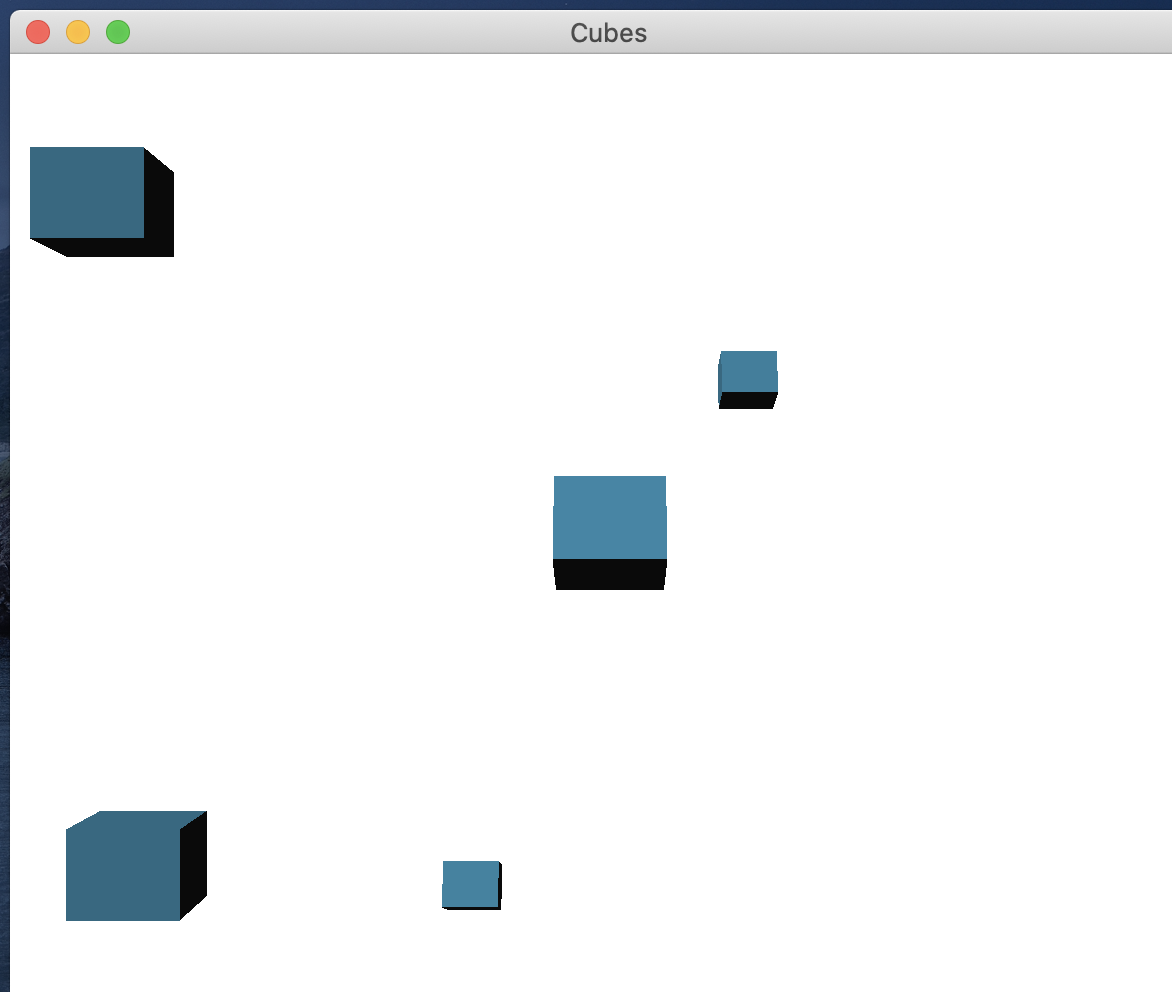
\includegraphics[scale=0.2]{basic.png}			
			\caption{Basic rigid body dynamics}
		\end{figure}
		\item Collision detection (we can set the system "paused" when a collision is detected, so that we can get this screenshot)
		\begin{figure}[H]
			\centering
			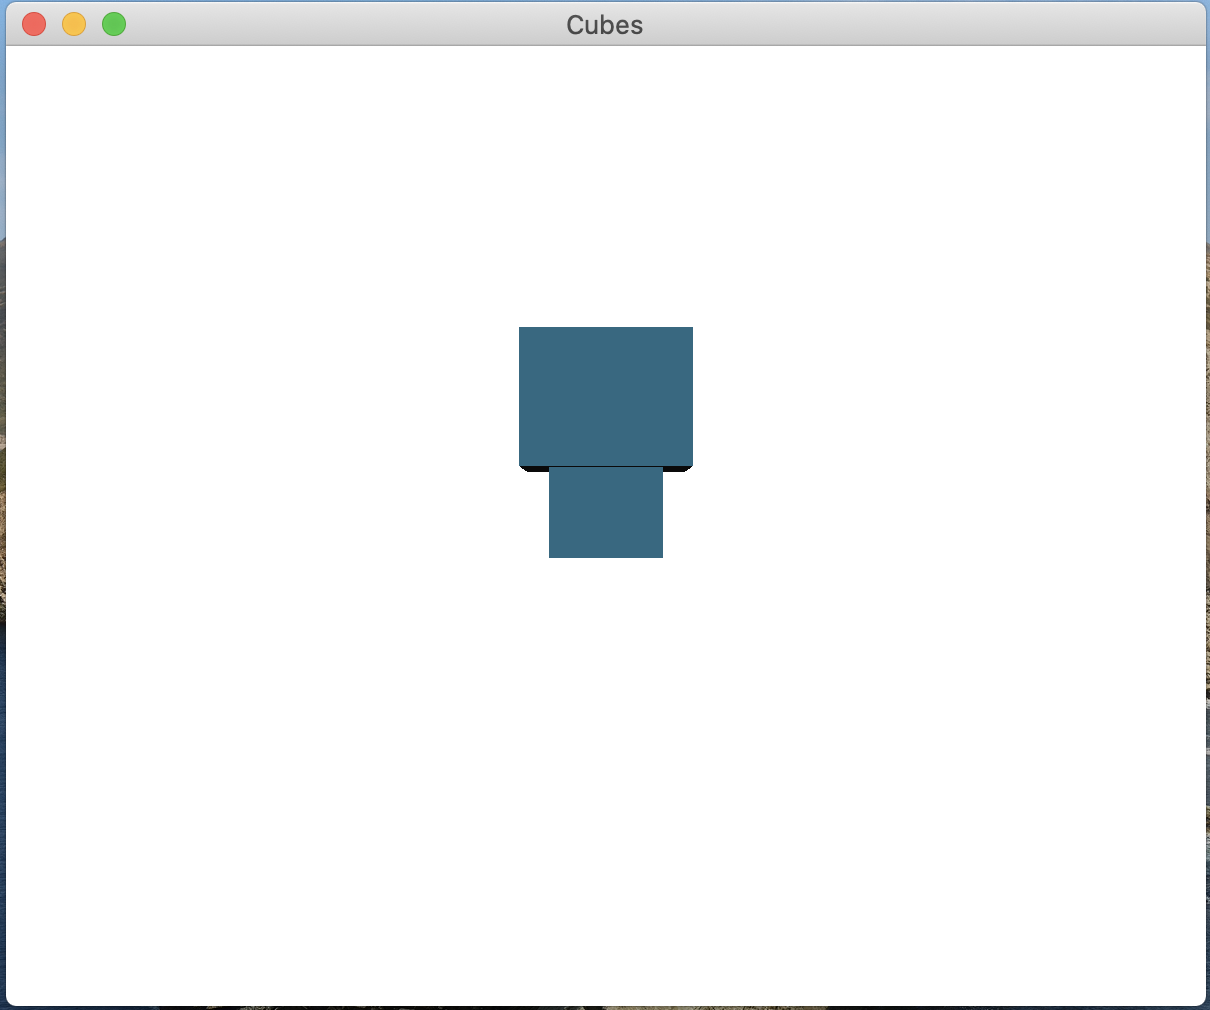
\includegraphics[scale=0.2]{coll1.png}			
			\caption{Collision detection}
		\end{figure}
		\begin{figure}[H]
			\centering
			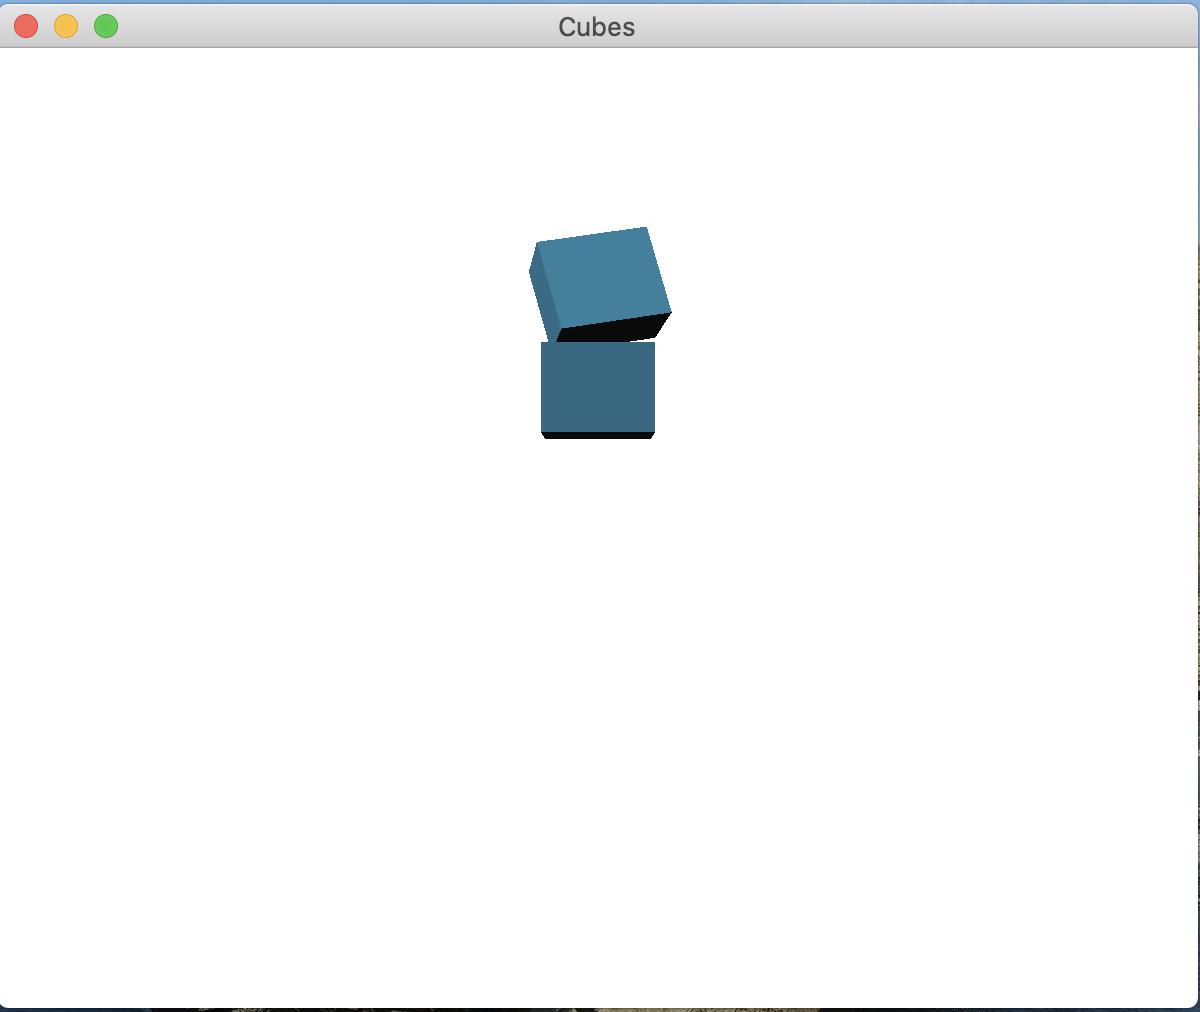
\includegraphics[scale=0.2]{coll2.png}			
			\caption{Collision detection}
		\end{figure}
		\item Collision contact handling. This figure shows the position and orientation of 
		these 2 cubes after collision occured.
		\begin{figure}[H]
			\centering
			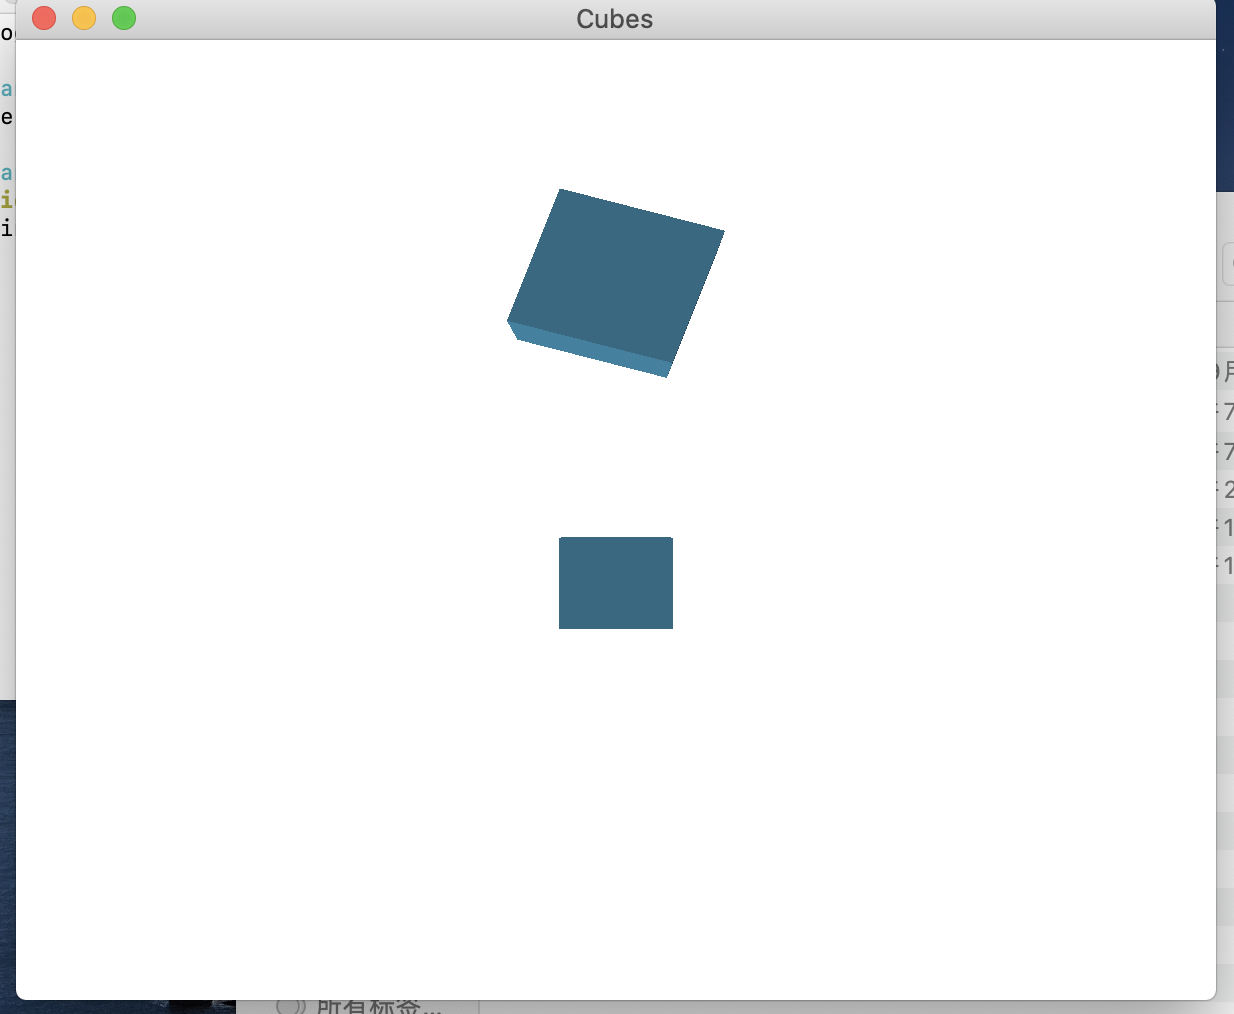
\includegraphics[scale=0.2]{collresp.png}			
			\caption{Collision contact handling}
		\end{figure}
	\end{enumerate}
	For the performance, the FPS (frame per second) of my engine can reach \~60fps under \~10 cubes (test platform is Intel i5-9400f and 
	macOS 10.15, the calculation is done single-threaded, and the complier is \texttt{Apple clang 12.0.0}.
\end{document}
